\section{Системы управления лифтами}

	Лифтовые механизмы подъема различаются по типам электроприводов.

	Одним из типов является нерегулируемый привод, в котором используется одно- и двухскоростные двигатели
		переменного тока. Такой привод используется в тихоходных лифтах с достаточно низкими требованиями
		к точности остановки кабины. 

	Другим типов привода является двухскоростной асинхронный привод.
		В нем используют двигатель с короткозамкнутым ротором и двумя статорными обмотками большой и малой скорости. 

	Также существует регулируемый привод постоянного тока, обеспечивающий аналогичные условия и использующийся
		при формирования схемы движения кабины лифта, близкой к оптимальной, и имеющий высокую точность остановки кабины.

	В современных лифтовых устройствах используются два принципа управления: замкнутый и разомкнутый.
		При использовании разомкнутого принципа управление приводом лебедки происходит с помощью сигналов,
		формируемых в логической управляющей системе. В данном случае не учитываются возможные изменения
		параметров лифта (лебедки и кабины) в процессе работы.

	При замкнутом принципе система позволяет учитывать все возможные изменения параметров и управлять приводом
		согласно сигналам, направленных от логической управляющей системы, более того, она позволяет учитывать
		результаты функционирования привода. Такая система управления дает возможность увеличить точность остановки,
		повысить плавность движения кабины.

    Замкнутый контур контроля скорости гарантирует точное и комфортное поведение привода в каждый момент работы. Измеренная скорость       электродвигателя вводится в регулятор скорости типа ПИ-регулятора. Динамическая точность регулирования скорости (время             устранения системой регулирования ошибки по скорости) высока.
    
	По видам функционального управления движением кабины лифты подразделяются на следующие типы:
		\begin{itemize}
			\item[--] внутренняя кнопочная система, осуществляющая вызов пустой кабины на любой этаж;
			\item[--] внутренняя кнопочная система, осуществляющая вызов пустой кабины на любой этаж,
				при этом совершая попутные остановки по вызовам при движении кабины вниз;
			\item[--] внутренняя кнопочная система, осуществляющая вызов пустой кабины на любой этаж,
				с попутными остановками по вызову при движении кабины вниз, с использованием группового управления;
			\item[--] собирательная внутренняя кнопочная система, осуществляющая вызов пустой кабины на любой этаж,
				с попутными остановками по вызову при движении кабины в любом направлении;
			\item[--] собирательная внутренняя кнопочная система, осуществляющая вызов пустой кабины на любой этаж,
				с попутными остановками по вызову при движении кабины  в любом направлении,
				а также с использованием группового управления.
		\end{itemize}
        
    Для пользовательского управления движением кабины лифта ипользуются кнопочные посты управления - вызывной и приказной пост.             Внешний вид постов управления представлен на рисунке \ref{dk2}.
    
     \begin{figure}[h]
				\centering
				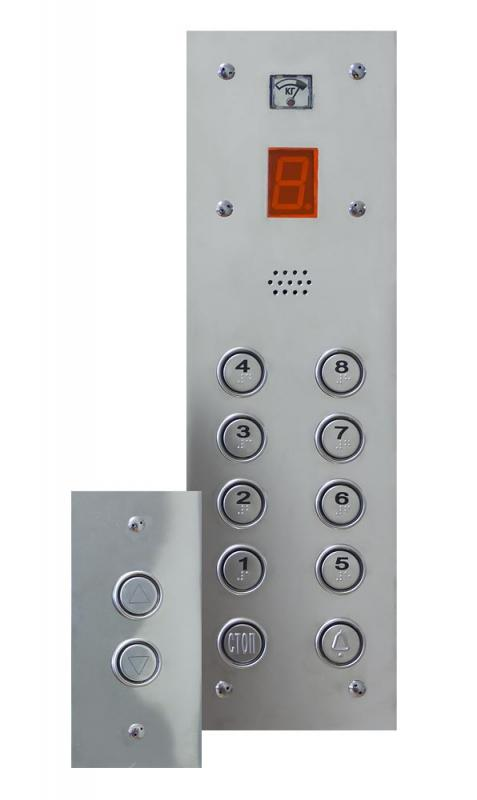
\includegraphics[width=90mm]{src/pictures/posti_upravlenia.jpg}
				\caption{Вызывной пост (слева) и приказной пост (справа)}\label{dk2}
    \end{figure}
		% Рис. 2 - Вызывной пост (слева) и приказной пост (справа)

	Самый простой вид управления, осуществляющий вызов пустой кабины на любой этаж,
		применяется для пассажирских лифтов грузоподъемностью до 320 кг,
		которые устанавливаются в жилых домах средней этажности (9-12 этажей).
		Как правило такие лифты монтируются по одному в подъезде, реже - по два в одной или рядом расположенных шахтах. 

	Все остальные виды управления используются для пассажирских лифтов грузоподъемностью 320-500 кг,
		устанавливаемых в домах повышенной и большой этажности (16 этажей и более),
		а также в административных зданиях. Такие лифты обычно монтируются по два и более в одной
		или рядом расположенных шахтах и работают в системе парного или группового управления.
